\documentclass[12pt,letterpaper,noanswers]{exam}
\usepackage[usenames,dvipsnames,svgnames,table]{xcolor}
\usepackage[margin=0.9in]{geometry}
\renewcommand{\familydefault}{\sfdefault}
\usepackage{multicol}
\pagestyle{head}
\header{AM 111 Class 20}{}{Discrete Fourier transform, p.\thepage}
\runningheadrule
\headrule
\usepackage{siunitx}
\usepackage{graphicx} % more modern
\usepackage{amsmath} 
\usepackage{amssymb} 
\usepackage{hyperref}
\usepackage{tcolorbox}
\usepackage{enumitem}
\def\mbf{\mathbf}
\newcommand{\vc}[1]{\boldsymbol{#1}}
\def\dsst{\displaystyle}
\DeclareMathOperator*{\argmin}{arg\,min} % thin space, limits underneath in displays
\usepackage[numbered,autolinebreaks,useliterate]{mcode}

\begin{document}
 \pdfpageheight 11in 
  \pdfpagewidth 8.5in

\noindent 

\section*{Preliminaries}

\begin{itemize}
\itemsep0pt
\item Your out of class assignment this week is project work.
\item There is a skill check in the next class.
\item Sarah's OH are cancelled today - find me on Ed.
\end{itemize}


\noindent\textbf{Big picture}

Today: Decomposing data using sinusoidal functions (Fourier methods).

\vspace{0.2cm}
\hrule
\vspace{0.2cm}

\noindent \textbf{Skill check practice}
\begin{questions}
\item There are $s = 132300$ data points in a data set with $3$ seconds of data.  Find the frequency associated with the $33$rd Fourier mode ($c_{33}$) in units of $1/$seconds (Hertz).

\item The skill from the Class 17 handout (Skill Check C18).
\end{questions}


\vspace{0.2cm}
\hrule
\vspace{0.2cm}

\noindent \textbf{Skill check solution}
\begin{questions}
\item This is the frequency associated with $33$ cycles (cosine or sine waves) in time $3$ seconds, which is $11$ cycles per second, or $11$ Hertz $(33/3)$.
\item See the past handout.
\end{questions}
\vspace{0.2cm}
\hrule
\vspace{0.2cm}

\noindent \textbf{Teams}
\begin{multicols}{3}
1. Mina, Ivonne, Emma

2.  RJ, Johan, Shang

3. Benjamin, Julia K, Dani

4. Nini, Mack, Daniyal

5. Kevin G, Julia M, Nina

6. Jack, Caitlin, Esmé

7. Cameron, Robert, Tom

8. Ray, Alex H, Jessica

9. Eli, Basil, Zachary

10.  Kevin C, Eric, Brian

11. Eletria, Sophia, Aidan

12. Alex B, Nicolas, Marissa

\end{multicols}


\section*{Ordinary differential equations}
\begin{tcolorbox}
To assess stability of the method, use the test equation $dy/dt = \lambda y$, with $\lambda \in \mathbb{C}$.
\begin{itemize}
\itemsep0pt
\item For $\lambda = a + ib$ with $a,b\in\mathbb{R}$, the exact solution to the test equation is $y(t) = y_0e^{\lambda t} = y_0e^{at}e^{ibt} = y_0e^{at}(\cos bt + i \sin bt)$.  It decays to $0$ for $a<0$, which corresponds to the left half of the complex plane.
    \item Apply a numerical method, with step size $h$, to the test equation.  Find the set of $h\lambda \in \mathbb{C}$ such that $y_k\rightarrow 0$ as $k\rightarrow\infty$.
    \item This is the region of \textbf{absolute stability} of the method.
    \item A method is called \textbf{A-stable} when the entire left half plane is in its region of absolute stability.
\end{itemize}
\end{tcolorbox}
\begin{enumerate}[resume=classQ]
    \item You applied the forward Euler method to $dy/dt = cy$ in the last class.  For this method, with $dy/dt = \lambda y$, $y_{k+1} = y_0(1+h\lambda)^{k+1}$.  
    \begin{parts}
    \item Find a mathematical expression for the region of absolute stability (the set of $h\lambda \in \mathbb{C}$ such that $y_k\rightarrow 0$ as $k\rightarrow \infty$).
 
 Answer is from last class: $y_k \rightarrow 0$ when $\vert 1+h\lambda \vert < 1$.
 
\item To help you plot this region in the complex plane, write $h\lambda = x + iy$, and find the set of points $(x,y)$ that satisfy the condition.

Answer is from last class: $\vert 1 + h\lambda \vert < 1$ becomes $\vert 1+ x+ iy\vert <1$ where $\vert (1+x) + iy\vert = \sqrt{(1+x)^2 + y^2}$.  Thus $\vert 1 + h\lambda \vert < 1$ is equivalent to

$(1+x)^2 + y^2 < 1$.  This is a disk in the complex plane (the real-imaginary plane), centered at $(-1,0)$ with radius $1$.

    \end{parts}


    \item Apply the backwards Euler method to the test equation.
    \begin{parts}
    \item First find an expression for $y_{k+1}$ in terms of $y_k$.  Then find an expression for $y_{k+1}$ in terms of $h,\lambda,k, y_0$.
    \vspace{1in}
    \item Find a mathematical expression for the region of absolute stability.
    \vspace{1.5cm}
    \item To help you think about this region in the complex plane, again write $h\lambda = x + iy$.  Argue that for $x<0$ the condition you found will always be true.
    \vspace{1in}
    \end{parts}
    The backwards Euler method is A-stable.
\end{enumerate}
\section*{Discrete Fourier transform (see Sauer \S 10)}
%Relates to: interpolation, least squares fitting.

\begin{tcolorbox}
\begin{itemize}
\itemsep0pt
    \item A sound wave is a sum of varying amounts of different frequencies.
    \item To represent the sound wave, let $\vc{x} = [x_0,...x_{n-1}]^T$ represent its volume at $n$ points that are evenly spaced in time.
\end{itemize}
\end{tcolorbox}
\hspace{-0.2in}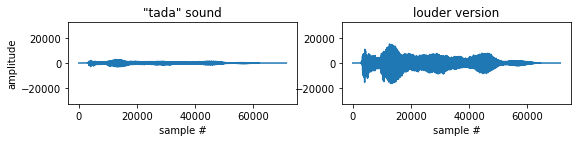
\includegraphics[width=0.7\linewidth]{img/C20tada.png}


\begin{tcolorbox}
\begin{itemize}
\itemsep0pt
    \item Write the sound wave sample, $\vc{x}$, as $\vc{x} = \sum\limits_{k=0}^{n-1}y_k \vc{w}_n^{(k)}$, where $\left\{\vc{w}_n^{(k)}\right\}_{k=0}^{n-1}$ is the \textbf{discrete Fourier basis} and each $k$ corresponds to a different frequency.
    \item $y_k$ is a complex number that encodes the amount of each frequency present in the sound wave, $\vert y_k\vert$, as well as the phase of that frequency (the angle of $y_k$ in the complex plane).
\end{itemize}



\end{tcolorbox}

\hspace{-0.1in}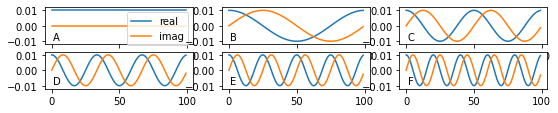
\includegraphics[width=\textwidth]{img/C20modes.png}

\begin{enumerate}[resume=classQ]
\item Six of the basis functions, $\left\{\vc{w}_n^{(0)}, \vc{w}_n^{(0)}, \vc{w}_n^{(1)}, \vc{w}_n^{(2)}, \vc{w}_n^{(3)}, \vc{w}_n^{(4)}, \vc{w}_n^{(5)}\right\}$, are plotted above.  Each basis function has a real part (a cosine wave) and an imaginary part (a sine wave).

\begin{parts}
\item Plot A1 is the sum of the sinusoids in A2.  Plot B1 is the sum of the sinusoids in B2.

Which $y_k$ are nonzero for A1?  \emph{The same $y_k$ are also nonzero for B1}.
\vspace{1cm}

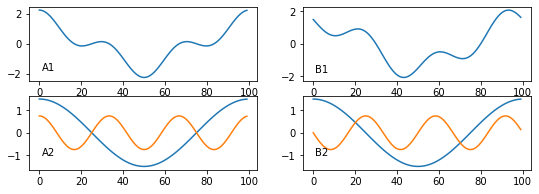
\includegraphics[width=0.7\textwidth]{img/C20modesadd.png}

\item One of the nonzero $y_k$ has an amplitude of $150$ and the other has an amplitude of $75$.  Which is which?
\vspace{1cm}
\item Each $y_k$ is either purely real or purely imaginary.  For each of A1 and B1 identify which $y_k$ are real and which are imaginary.
\vspace{1cm}
\end{parts}
\end{enumerate}

\begin{tcolorbox}
\begin{itemize}
\itemsep0pt
    \item A \textbf{discrete Fourier transform} (DFT) allows you to find the $y_k$ given a signal $\vc{x}$.
    \item Let $\vc{y} = [y_0, y_1,...,y_{n-1}]^T$.  The \textbf{inverse DFT} allows you to find $\vc{x}$ given the set of weights $\vc{y}$ in frequency space.
\end{itemize}
\end{tcolorbox}
\begin{tcolorbox}
\begin{itemize}
\itemsep0pt
     \item The DFT is given by
     
    \[\vc{y} =F_n\vc{x}\] where
    \[F_n =  \left[\begin{array}{l l l l l}
    \omega^0 & \omega^0 &\omega^0 & \hdots & \omega^0 \\
    \omega^0 & \omega^{1} & \omega^{2} & \hdots & \omega^{n-1} \\
    \omega^0 & \omega^{2} & \omega^{4} & \hdots & \omega^{2(n-1)}\\
    \vdots & \vdots & \vdots & & \vdots \\
    \omega^0 & \omega^{n-1} & \omega^{2(n-1)} & \hdots &\omega^{(n-1)^2}
    \end{array}\right]\]
    and  $\omega = e^{-2\pi i/n} = \cos(2\pi/n) - i\sin(2\pi/n)$.
    \item 
    %From $\vc{x} = \sum\limits_{k=0}^{n-1}y_k \vc{w}_n^{(k)}$, 
    The inverse DFT is given by 
 \[\vc{x} = F_n^{-1}\vc{y}\]
 where \[F_n^{-1} = \dfrac{1}{n} \left[\begin{array}{l l l l l}
    \omega^0 & \omega^0 &\omega^0 & \hdots & \omega^0 \\
    \omega^0 & \omega^{-1} & \omega^{-2} & \hdots & \omega^{-(n-1)} \\
    \omega^0 & \omega^{-2} & \omega^{-4} & \hdots & \omega^{-2(n-1)}\\
    \vdots & \vdots & \vdots & & \vdots \\
    \omega^0 & \omega^{-(n-1)} & \omega^{-2(n-1)} & \hdots &\omega^{-(n-1)^2}
    \end{array}\right]\]
%  %\left[\vc{w}_n^{(0)}, \vc{w}_n^{(1)},...,\vc{w}_n^{(n-1)}\right]\vc{y}\]
%  \item $\vc{w}_n^{(k)} = \dfrac{1}{n}\left[\omega^{0k}, \omega^{-k}, \omega^{-2k}, \omega^{-3k},...,\omega^{-(n-1)k}\right]^T$ 
  
\end{itemize}
The choice of how to incorporate the factor $1/n$ is not standardized.  For example, it is sometimes split as a factor of $1/\sqrt{n}$ on both $F_n$ and $F_n^{-1}$.  The choice above is made to match \texttt{scipy.fft}.
\end{tcolorbox}


\begin{enumerate}[resume=classQ]
    \item That $F_n^{-1}$ is the inverse of $F_n$ is not obvious.  Let $a_{jk}$ be the $(j,k)$ entry in $F_n^{-1}F_n$.
    \begin{parts}
    \item Consider the diagonal entries, $a_{kk}$.  These are given by \[\dfrac{1}{n}\left[\omega^0, \omega^{-k},\omega^{-2k},\hdots,\omega^{-k(n-1)}\right]\left[\begin{array}{l}
    \omega^0\\
    \omega^{k}\\
    \omega^{2k}\\
    \vdots\\
    \omega^{k(n-1)}
    \end{array}\right]\]
    
    Show that the diagonal terms are $1$.
    \vspace{1in}
    
    \item Now we need to show that the off-diagonal terms are $0$.  
    
    \[\dfrac{1}{n}\left[\omega^0, \omega^{-j},\omega^{-2j},\hdots,\omega^{-j(n-1)}\right]\left[\begin{array}{l}
    \omega^0\\
    \omega^{k}\\
    \omega^{2k}\\
    \vdots\\
    \omega^{k(n-1)}
    \end{array}\right]\]
    
    Find an appropriate $c$ and write this as $\dfrac{1}{n}\left(1 + \omega^{c}+\omega^{2c} + ... + \omega^{c(n-1)}\right)$.
    \vspace{1cm}
    \item $\omega$ is the $n$th root of unity.  Use Euler's formula ($e^{ix} = \cos x + i\sin x$) to convince yourself that $\omega^n = 1$.
    \vspace{1cm}
    \item For $1\leq c < n$, show that
    $(1-\omega^c)(1+\omega^c + \omega^{2c} + \omega^{3c} + ... + \omega^{c(n-1)}) = 1-\omega^{cn}$.
    \vspace{1in}
    \item Given that $\omega^n = 1$, $\omega^{cn} = 1$, and $\omega^c \neq 1$, what can you conclude about $1+\omega^c + \omega^{2c} + \omega^{3c} + ... + \omega^{c(n-1)}$?
    \vspace{1in}
    
    \end{parts}
\end{enumerate}
\subsection*{DFT and interpolation (Sauer \S 10.2)}
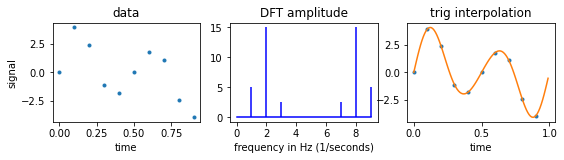
\includegraphics[width=0.9\linewidth]{img/C20interp.png}
\begin{tcolorbox}
\begin{itemize}
\itemsep0pt
    \item Let $\vc{x}$ be real-valued data sampled at evenly spaced points $\vc{t}$ on the interval $[0,1)$, with sample points $t_j = j/n$ for $j=0,...,n-1$.
    \item Let $\vc{y}$ be the DFT of the data.  $\vc{x} = F_n^{-1}\vc{y}$: the sum of the Fourier modes (using weights $\vc{y}$) passes through the data points exactly.
\end{itemize}
\end{tcolorbox}
% \begin{enumerate}[resume=classQ]
% \item For the data in the plot above, the $y_k$ are given by $\vc{y} = \left[\begin{array}{r} 0 \\-5i, \\-15i\\ -2.5i\\ 0\\ 0\\ 0\\ -2.5i\\ -15i\\ -5i\end{array}\right]$
% \begin{parts}
% \item At a frequency of $1$ (a single period in the interval $[0,1)$, $y_1 = -5i$.  The associated trigonometric function is $\frac{1}{10}\cos (2\pi t)+i\sin(2\pi t)$.

% \end{parts}
% \end{enumerate}
\begin{enumerate}[resume=classQ]
\item \[\vc{x} = \sum\limits_{k=0}^{n-1} y_k \frac{1}{n}\left[\begin{array}{l} \omega^0 \\\omega^{-k} \\\omega^{-2k}\\
\vdots \\
\omega^{-k(n-1)}\end{array}\right] = \sum\limits_{k=0}^{n-1} y_k \frac{1}{n}\left[\begin{array}{l} e^{2\pi i (0/n)} \\e^{2\pi ki (1/n)} \\e^{2\pi ki (2/n)}\\
\vdots \\
e^{2\pi ki ((n-1)/n)}\end{array}\right] = \sum\limits_{k=0}^{n-1} y_k \frac{1}{n}\left[\begin{array}{l} e^{2\pi ki t_0} \\e^{2\pi ki t_1} \\e^{2\pi ki t_2}\\
\vdots \\
e^{2\pi ki t_{n-1}}\end{array}\right]\]
\begin{parts}
\item Think of the vector \[\frac{1}{n}\left[\begin{array}{l} e^{2\pi ki t_0} \\e^{2\pi ki t_1} \\e^{2\pi ki t_2}\\
\vdots \\
e^{2\pi ki t_{n-1}}\end{array}\right]\] as a complex function, $g_k$, evaluated at the time points $\vc{t}$.  Write down $g_k$.
\vspace{1in}
\item Let $y_k = a_k + i b_k$.  Find the real part of $(a_k + ib_k)g_k$.
\vspace{1in}
\item The real function $P(t)$, given by the real part of $\sum\limits_{k=0}^{n-1} y_kg_k(t)$, uses the weights $y_k$ as interpolation coefficients on trig functions.  Use your result from (b) to write an expression for $P(t)$.
\vspace{0.7in}
\end{parts}
\end{enumerate}
\subsection*{(extra fact) DFT and least squares (Sauer \S 10.3.2)}
\begin{tcolorbox}
\begin{itemize}
\itemsep0pt
    \item Consider the trigonometric least squares problem, where $m$ basis functions (with indices $S = \{j_0,j_2,...,j_{m-1}\}$) are chosen for least squares fitting from the $g_k(t)$ above.
    \item For $m<n/2$, this is a compression problem.
    \item $P_m(t) = \sum\limits_{k=0}^m y_{j_k}g_{j_k}(t)$.  The error vector, $\vc{e} = P(\vc{t}) - P_m(\vc{t}) = \sum\limits_{k\notin S}y_k g_k(\vc{t})$.  The vectors formed by $g_k$ evaluated at $\vc{t}$ are orthogonal, so $\vc{e}$ is orthogonal to the span of $\left\{g_{j_k}(\vc{t})\right\}_{j_k\in S}$.  i.e. $P_m(t) = \sum\limits_{k=0}^m y_{j_k}g_{j_k}(t)$ is the least squares solution.
\end{itemize}
\end{tcolorbox}
% \begin{enumerate}[resume=classQ]
% \item $\vc{e} = \left\{P(t_j) - P_m(t_j)\right\}_{j=0}^{n-1}$.  Argue that this error vector is orthogonal to the span of $g_{j_k}(t_j)$
% \end{enumerate}
% %\item Let there be four data points on $[0,1)$: $(0,1)$, $(0.25, 0)$, $(0.5,-1)$, $(0.75,0)$.
% \end{enumerate}
\end{document}